\documentclass{article}
\usepackage[utf8]{inputenc}
\usepackage{algorithm}
\usepackage{algpseudocode}
\usepackage{graphicx}
\usepackage{wrapfig}
\usepackage{geometry}
 \geometry{
 a4paper,
 total={170mm,257mm},
 left=20mm,
 top=20mm,
 }
\title{Drug Consumption: A Machine Learning Analysis of Marijuana 
and Other Drug Users}
\author{Priyanshi Aeron, Samantha Anthony, Zachary Hudgins, Tarini Ramesh}
\date{}

\begin{document}

\maketitle

\section{Introduction}

\section{Literature Review}

\section{Study Data}

\section{Methodology}
In order to answer our question of [insert question], we generated and tuned many different models. We modeled logistic classification, support vector machine, random forest, and a neural network due to their prominence and historic aptitude for binary classification tasks.
\subsection{Logistic Classification}
\subsection{Support Vector Machine}
\subsection{Random Forest}
The next model generated was a Random Forest model. A Random Forest is a powerful classifier that uses an ensemble of relatively uncorrelated decision trees which are then used as a whole to vote on which class each data point belongs to. To begin, we started from the bottom by building a single decision tree to get a baseline of how much our base model could stand to improve. This resulted in a base model accuracy of 0.848 and an AUC, or area under the receiver operating characteristic (ROC) curve, of 0.795. Next, we generated a base model for a random forest, which resulted in an accuracy of 0.8963 and AUC of 0.948. Since an AUC of 1.0 means perfect classification, and the random forest’s AUC was higher, it is easy to conclude that the random forest was better than just the single decision tree. However, even with these strong accuracy and AUC measurements, the random forest could be improved by some parameter tuning. To tune the hyperparameters, the metric we aimed to minimize was the out-of-bag (OOB) error, a standard measure of prediction error for random forests using bootstrapping, which averages prediction error on observations not used to generate the next tree. The hyperparameters that were tuned were the splitting criteria for each node, number of features for best split, maximum depth of the individual trees, and number of decision trees in the forest. Various values for each of these hyperparameters were tested against different random forests of many sizes. This hyperparameter tuning is displayed in the graphs and interpreted below.

\begin{figure}[htp]
    \centering
    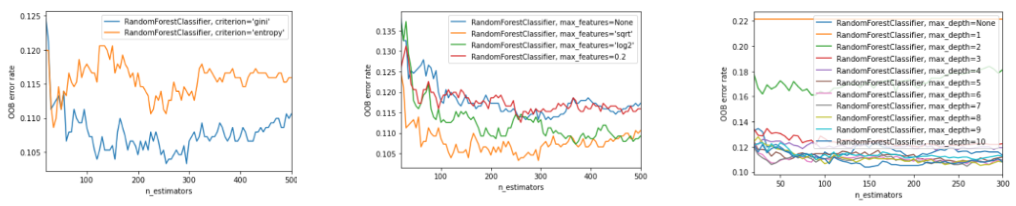
\includegraphics[width=12cm]{RF_hyperparameter_tuning.png}
    \label{fig:randforest}
\end{figure}

\noindent From the first graph, we can conclude that gini is the better criterion to minimize OOB error at larger values of the number of estimators used for the random forests. Additionally, the optimal maximum features parameter is the square root because it stabilizes to the lowest OOB error at the larger numbers of estimators. From the final graph, the maximum tree depths above around four all begin to converge to a very small OOB error, therefore the default parameter of no max depth was chosen because it produced the same results as the other depths. Finally, all of these values converged to low OOB errors around 150 to 300 decision trees, or estimators, in the forest, so the number of 250 decision trees was chosen due to it being in the range and not drastically increasing model computation time. After all the hyperparameter tuning, the model generated resulted in an accuracy of 0.915 and an AUC of 0.955. Therefore, the new tuned model was more accurate and had a larger AUC than the base models before, meaning it was a better model for the data.

\subsection{Neural Network}

\section{Results}
\begin{wrapfigure}{r}{7.4cm}
  \centering
  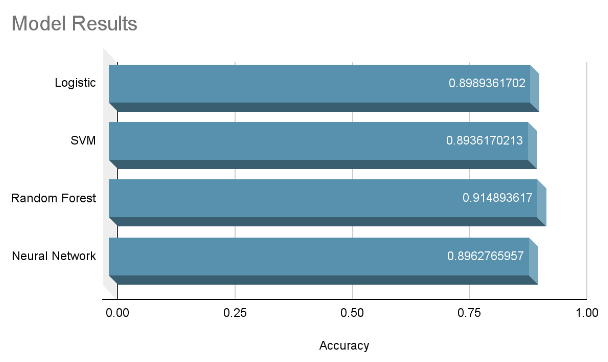
\includegraphics[height=3.7cm]{model_results.png}
\end{wrapfigure}
The models generated to answer our question were all decent models, as described above. They were all able to predict labels on the test set fairly well. As evident in the Model Results figure, the model that produced the most accurate classification was the Random Forest. It is worth noting that all the models had around 0.90 accuracy and similarly high precision. However, due to its higher accuracy and in-depth analysis features, the Random Forest model was chosen as our best model to solve this task. 
After testing the optimized model, the random forest resulted in an AUC of 0.955 and an accuracy of 0.915 on the test set. The ROC curve and confusion matrix are displayed above, in order. Following the creation and verification of that model, we started looking into how the random forest was able to conclude who was a marijuana user and who had never used it. To do so, we looked at feature importance.
\begin{figure}[htp]
\centering
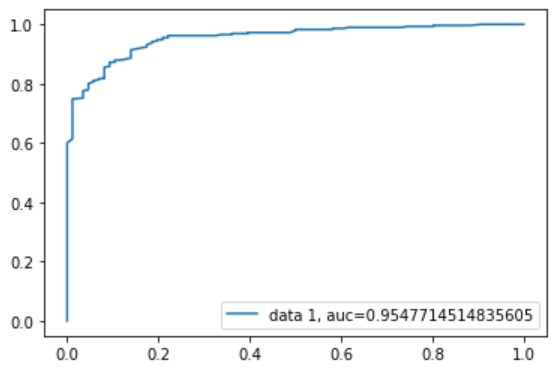
\includegraphics[width=.2\textwidth]{rf_auc_curve.png}\hfill
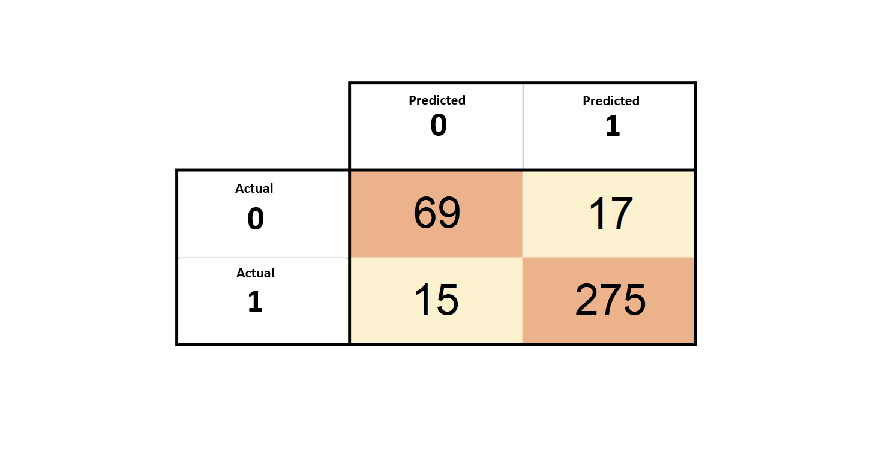
\includegraphics[width=.2\textwidth]{rf_conf_matrix.png}\hfill
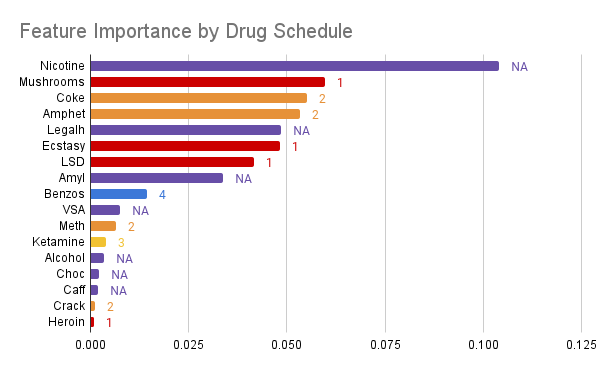
\includegraphics[width=.3\textwidth]{Feature Importance by Drug Schedule.png}\hfill
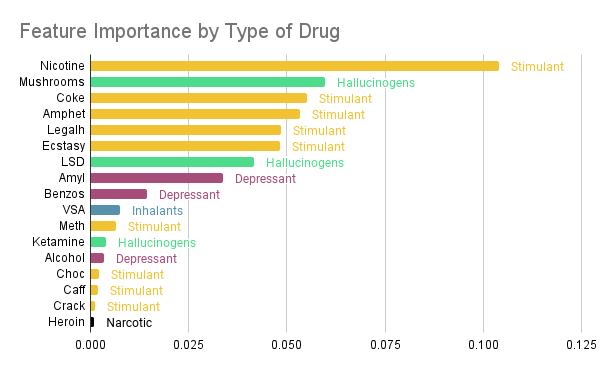
\includegraphics[width=.3\textwidth]{Feature Importance by Type of Drug.png}
\end{figure}

According to the model, the most important determining factor of whether or not a participant was a marijuana user was if they used nicotine. This aligns with previously conducted research on marijuana users and nicotine smokers. This relationship could be due to the fact that these drugs are easily accessible, however other easily accessible drugs like alcohol or caffeine were not important features. Therefore, there is something about nicotine that is specifically correlated to marijuana use, such as their documented interactive effects. Next, we colored the feature importances according to which schedule the drug is, as determined by the United States Drug Enforcement Administration. As you can see in the chart above, marijuana (schedule 1) did not simply lead to other schedule 1 or 2 drugs as a whole. In fact, heroin, a major schedule 1 drug, and meth, a major schedule 2 drug, are not significantly related to marijuana use, according to the model. Some of the primary features that help predict marijuana use are actually unscheduled. Therefore, one cannot conclude that marijuana use will automatically lead to using major schedule 1 drugs as a whole. Finally, we looked into the types of drugs that were correlated with marijuana use in the above graph on the right. Marijuana is a hallucinogen and stimulant, resulting in the hypothesis that weed use would lead to similar drug use. This hypothesis is supported by the figure which shows a high correlation between marijuana use and other hallucinogens and stimulants, such as nicotine, mushrooms, and cocaine. Instead of leading to depressants or narcotics, marijuana use was primarily correlated to users of similar hallucinogenic and stimulant drugs.

\section{Future Research}

\section{Conclusion}

\end{document}

